\chapter*{Caracterización del GRID}
\addcontentsline{toc}{chapter}{Caracterización del GRID}\label{cap:caracterizacionGRID}
El Grupo de Investigación en Redes, Información y Distribución (GRID) de la Universidad del Quindío se dedica a la educación, 
investigación y extensión, siendo los objetivos misionales de la Universidad del Quindío. Desde el grupo de investigación se busca ofrecer servicios tecnológicos
a la comunidad académica, especialmente a los estudiantes de Ingeniería de Sistemas y Computación.

\section*{1.1 Análisis de stakeholders del grupo GRID}

Para comprender mejor las necesidades y expectativas del GRID, se realizó un análisis de los stakeholders involucrados. Este análisis incluyó a los miembros del grupo de investigación, estudiantes, 
docentes, entre otros, identificando sus roles, impacto y poder de influencia por una solución basada en las tecnologías de virtualización basadas en contenedores (VBC).

\begin{table}[H]
    \centering
    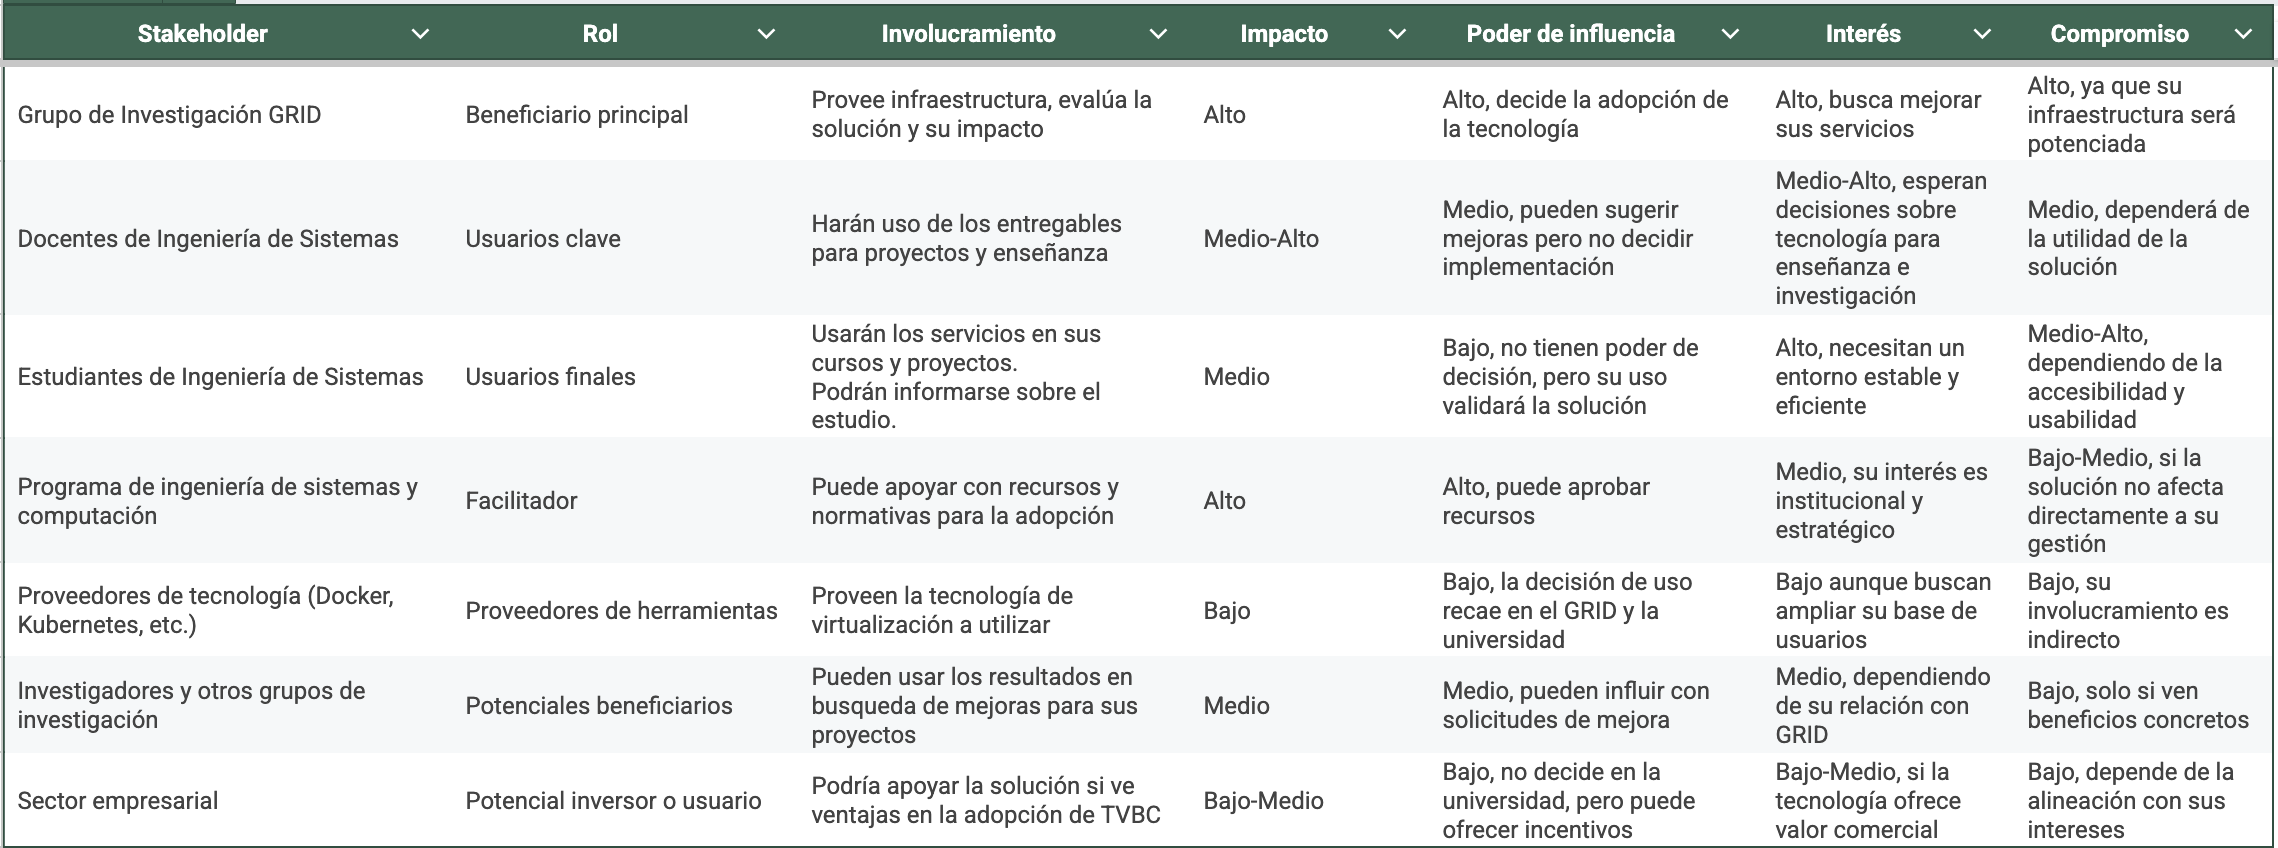
\includegraphics[width=\textwidth]{tablas-images/cp1/definicionStakeholders.png}
    \caption{Análisis de stakeholders del proyecto}
    \label{tab:tabla-stakeholders}
\end{table}

\section*{1.2 Priorización de stakeholders}
A partir del análisis de stakeholders, se priorizaron aquellos que tienen mayor impacto y poder de influencia en el proyecto. Esta priorización permite enfocar los esfuerzos de comunicación y gestión de expectativas hacia
los stakeholders más relevantes, asegurando que sus necesidades sean atendidas de manera especial.

\begin{figure}[H]
    \centering
    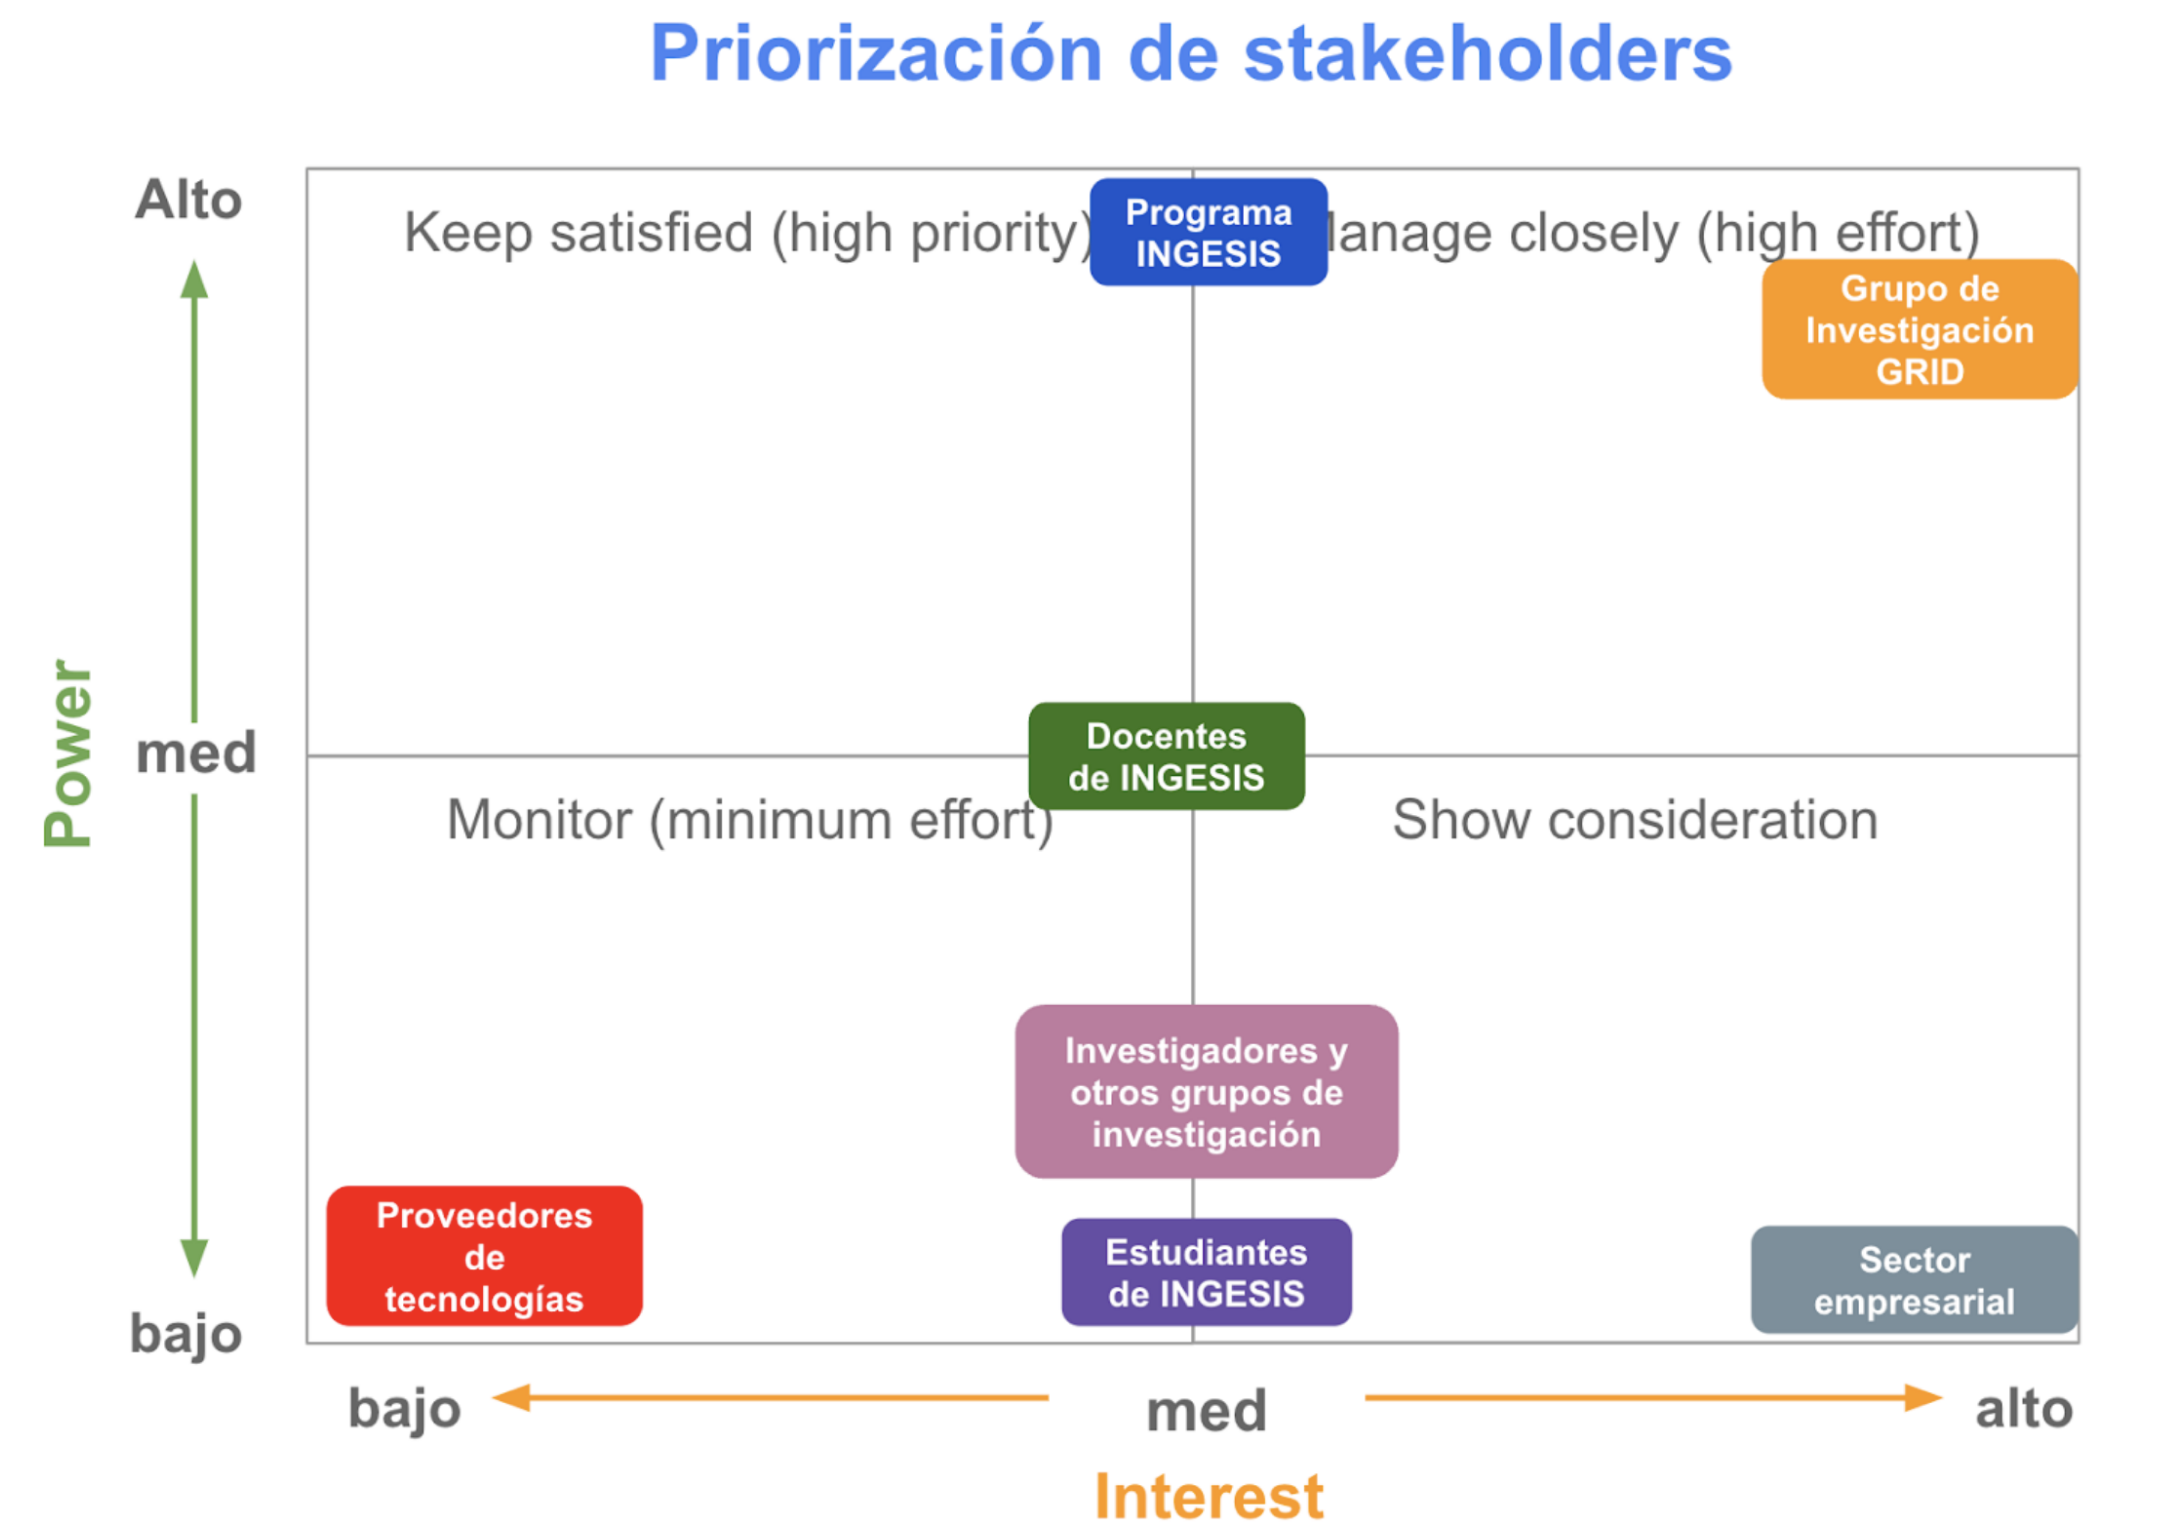
\includegraphics[width=\textwidth] {tablas-images/cp1/priorizacionStakeholders.png}
    \caption{Priorización de stakeholders del proyecto}\label{fig:tabla-priorizacion-stakeholders}
\end{figure}

\section*{1.3 Integrantes y áreas de trabajo del GRID}

El GRID está compuesto por un equipo multidisciplinario de investigadores y profesionales, cada uno con áreas de especialización diferentes. A continuación se presentan los diferentes integrantes y sus respectivas áreas de trabajo:

\begin{itemize}
  \item \href{https://scienti.minciencias.gov.co/cvlac/visualizador/generarCurriculoCv.do?cod_rh=0000210897}{\textbf{Christian Andrés Candela Uribe}}: Microservicios, desarrollo de software, minería de datos, infraestructura TI
  \item \href{https://scienti.minciencias.gov.co/cvlac/visualizador/generarCurriculoCv.do?cod_rh=0001383939}{\textbf{Luis Eduardo Sepúlveda Rodríguez}}: Infraestructura de TI, HPC, computación paralela
  \item \href{https://scienti.minciencias.gov.co/cvlac/visualizador/generarCurriculoCv.do?cod_rh=0001638854}{\textbf{Carlos Andrés Flórez Villarraga}}: Programación y algoritmia, Activa, inteligencia artificial
  \item \href{https://scienti.minciencias.gov.co/cvlac/visualizador/generarCurriculoCv.do?cod_rh=0001343801}{\textbf{Carlos Eduardo Gómez Montoya}}: Networking, ingeniería de software, cloud computing
  \item \href{https://scienti.minciencias.gov.co/cvlac/visualizador/generarCurriculoCv.do?cod_rh=0001398775}{\textbf{Sergio Augusto Cardona Torres}}: Big data y análisis de datos, ingeniería de software, educación asistida por computador - sistemas adaptativos, informática educativa
  \item \href{https://scienti.minciencias.gov.co/cvlac/visualizador/generarCurriculoCv.do?cod_rh=0000193550}{\textbf{Sonia Jaramillo Valbuena}}: Big data, electroquímica, inteligencia artificial
  \item \href{https://scienti.minciencias.gov.co/cvlac/visualizador/generarCurriculoCv.do?cod_rh=0000283495}{\textbf{Julián Esteban Gutiérrez Posada}}: Microservicios, desarrollo de software, minería de datos, infraestructura TI, HPC, computación paralela, networking, ingeniería de software
\end{itemize}

\section*{1.4 Misión del GRID}
\addcontentsline{toc}{section}{1.4 Misión del GRID}

La misión del GRID es heredada de la Universidad del Quindío. A continuación se presenta la misión del GRID:

\begin{quote}
La Universidad del Quindío contribuye a la transformación de la sociedad, mediante la formación integral desde el ser, el saber y el hacer, de líderes reflexivos y gestores del cambio; con estándares de calidad, a través de una oferta de formación en diferentes metodologías, que responda a una sociedad basada en el conocimiento; una investigación pertinente, que aporte a la solución de las problemáticas del desarrollo e integrada con la extensión y proyección social; educando en tiempos del posconflicto y de la consolidación de la paz, apoyada en una gestión creativa y con estándares de calidad.
\end{quote}

A partir de esta misión, se identifican los siguientes pilares fundamentales:

\begin{itemize}
    \item \textbf{Docencia:} La Universidad del Quindío contribuye a la transformación de la sociedad, mediante la formación integral desde el ser, el saber y el hacer, de líderes reflexivos y gestores del cambio; con estándares de calidad, a través de una oferta de formación en diferentes metodologías, que responda a una sociedad basada en el conocimiento.

    \item \textbf{Investigación:} Una investigación pertinente, que aporte a la solución de las problemáticas del desarrollo e integrada con la extensión y proyección social.

    \item \textbf{Extensión y Desarrollo Social:} Apoyada en una gestión creativa y con estándares de calidad.

    \item \textbf{Responsabilidad Social:} Educando en tiempos del posconflicto y de la consolidación de la paz.
\end{itemize}

\section*{1.5 Visión del GRID}
\addcontentsline{toc}{section}{1.5 Visión del GRID}

\begin{quote}
En el año 2025, la Universidad del Quindío estará consolidada como una institución \textit{Pertinente - Creativa - Integradora}, acreditada de alta calidad, con reconocimiento nacional e internacional en sus procesos de formación a través de diferentes metodologías, de investigación, extensión, proyección y responsabilidad social.
\end{quote}

A partir de esta visión, se destacan los siguientes enfoques estratégicos:

\begin{itemize}
    \item \textbf{Gestión:} La Universidad del Quindío estará consolidada como una institución \textit{Pertinente - Creativa - Integradora}.

    \item \textbf{Docencia:} Acreditada de alta calidad en sus procesos de formación a través de diferentes metodologías.

    \item \textbf{Investigación:} Consolidada como pertinente y de alta calidad en sus procesos de investigación.

    \item \textbf{Extensión y Desarrollo Social:} Procesos creativos e integradores en proyección social.

    \item \textbf{Responsabilidad Social:} Reconocimientos en sus procesos de responsabilidad social.
\end{itemize}

\section*{1.6 Impacto del proyecto en el GRID}
\addcontentsline{toc}{section}{1.6 Impacto del proyecto en el GRID}

El proyecto tiene como objetivo apoyar los procesos de \textbf{docencia}, \textbf{investigación} 
y \textbf{extensión} mediante la especificación de una arquitectura de tecnologías de 
virtualización basada en contenedores (VBC). 

Este trabajo se enfoca en la identificación de una tecnología de contenerización que 
\textbf{agregue valor a los procesos del GRID}, beneficiando a \textbf{docentes}, \textbf{estudiantes} 
y cualquier parte interesada que participe en los proyectos y actividades desarrolladas 
por este grupo de investigación.

\section*{1.7 Caracterización de la infraestructura tecnológica del GRID}
En el siguiente formato se van a especificar las características técnicas de la infraestructura tecnológica del GRID disponible para temas de virtualización. \href{https://docs.google.com/spreadsheets/d/14NBv72ucVTrLqGIldYdIsjdBGt3QlgwcblcVRis-DaQ/edit?usp=sharing}{Macro de la ficha técnica}

% Archivo de caracterización de infraestructura corregido

% Torre HP 1
\begin{table}[H]
\centering
\caption{Ficha técnica --- Torre 1}\label{tab:torre-hp-1}
\begin{tabular}{|p{0.6\textwidth}|p{0.3\textwidth}|}
\hline
\multicolumn{2}{|l|}{\textbf{DESCRIPCIÓN FÍSICA:} Servidor tipo torre} \\ \hline
\textbf{TIPO DE RECURSO:} Torre &
\multirow{5}{*}{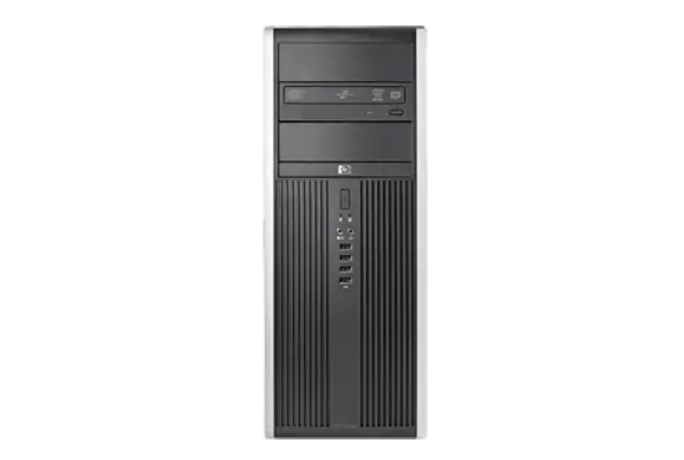
\includegraphics[width=0.25\textwidth,height=4cm,keepaspectratio]{tablas-images/cp1/torres/torre-1.png}} \\ \cline{1-1}
\textbf{MODELO:} Desconocido & \\ \cline{1-1}
\textbf{MARCA:} HP & \\ \cline{1-1}
\textbf{CÓDIGO DE INVENTARIO:} 7 24390 49867 3 & \\ \cline{1-1}
\textbf{NÚMERO EN CPD:} 14 & \\ \hline
\multicolumn{2}{|l|}{\textbf{ESPECIFICACIONES TÉCNICAS}} \\ \hline
\multicolumn{2}{|p{0.95\textwidth}|}{
\footnotesize
- 8 entradas USB (4 al frente, 4 en la parte trasera)
- Entrada de audio y microfono
- Entrada HDMI
- Lector de DVDs
- 3 puertos Ethernet (Parte trasera)
- Entrada Displayport
- Puertos PS/2 (Teclado y Ratón)
} \\ \hline
\multicolumn{2}{|l|}{\textbf{PROPÓSITO:} Hipervisor de XCP-ng} \\ \hline
\multicolumn{2}{|l|}{\textbf{OPORTUNIDAD DE USO:} Proyectos del \GRID} \\ \hline
\multicolumn{2}{|p{0.9\textwidth}|}{\textbf{OBSERVACIONES:} El Equipo no tiene modelo. El equipo está diseñado para usuario final pero fue adaptado para entornos de virtualización.} \\ \hline
\end{tabular}
\end{table}


% Torre 2
\begin{table}[H]
\centering
\caption{Ficha técnica --- Torre 2}\label{tab:torre-2}
\begin{tabular}{|p{0.6\textwidth}|p{0.3\textwidth}|}
\hline
\multicolumn{2}{|l|}{\textbf{DESCRIPCIÓN FÍSICA:} Servidor tipo torre} \\ \hline
\textbf{TIPO DE RECURSO:} Torre & 
\multirow{5}{*}{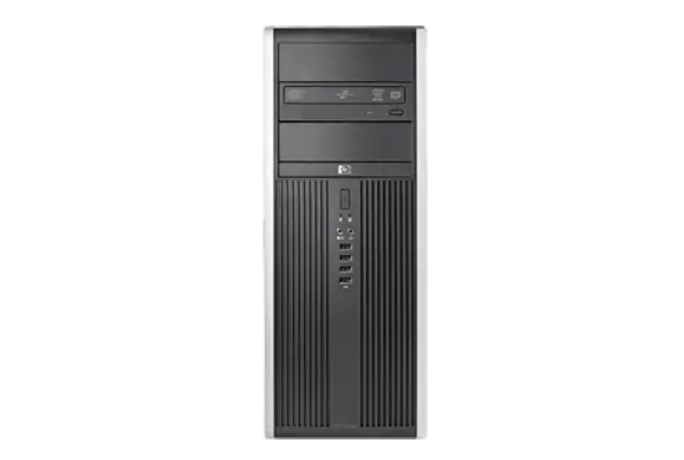
\includegraphics[width=0.25\textwidth,height=4cm,keepaspectratio]{tablas-images/cp1/torres/torre-1.png}} \\ \cline{1-1}
\textbf{MODELO:} Desconocido & \\ \cline{1-1}
\textbf{MARCA:} HP & \\ \cline{1-1}
\textbf{CÓDIGO DE INVENTARIO:} 7 24390 49861 1 & \\ \cline{1-1}
\textbf{NÚMERO EN CPD:} 12 & \\ \hline
\multicolumn{2}{|l|}{\textbf{ESPECIFICACIONES TÉCNICAS}} \\ \hline
\multicolumn{2}{|p{0.95\textwidth}|}{
\footnotesize
- 8 entradas USB (4 al frente, 4 en la parte trasera)
- Entrada de audio y microfono
- Entrada HDMI
- Lector de DVDs
- 3 puertos Ethernet (Parte trasera)
- Entrada Displayport
- Puertos PS/2 (Teclado y Ratón)
} \\ \hline
\multicolumn{2}{|l|}{\textbf{PROPÓSITO:} Hipervisor de XCP-ng} \\ \hline
\multicolumn{2}{|l|}{\textbf{OPORTUNIDAD DE USO:} Proyectos del \GRID} \\ \hline
\multicolumn{2}{|p{0.9\textwidth}|}{\textbf{OBSERVACIONES:} El Equipo no tiene modelo. El equipo está diseñado para usuario final pero fue adaptado para entornos de virtualización.} \\ \hline
\end{tabular}
\end{table}

% Torre 3
\begin{table}[H]
\centering
\caption{Ficha técnica -- Torre 3}
\label{tab:torre-3}
\begin{tabular}{|p{0.6\textwidth}|p{0.3\textwidth}|}
\hline
\multicolumn{2}{|l|}{\textbf{DESCRIPCIÓN FÍSICA:} Servidor tipo torre} \\ \hline
\textbf{TIPO DE RECURSO:} Torre & 
\multirow{5}{*}{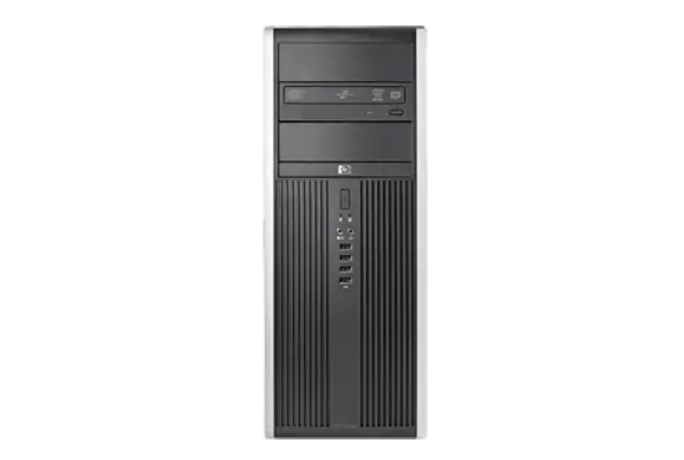
\includegraphics[width=0.25\textwidth,height=4cm,keepaspectratio]{tablas-images/cp1/torres/torre-1.png}} \\ \cline{1-1}
\textbf{MODELO:} Desconocido & \\ \cline{1-1}
\textbf{MARCA:} HP & \\ \cline{1-1}
\textbf{CÓDIGO DE INVENTARIO:} 7 24390 49969 4 & \\ \cline{1-1}
\textbf{NÚMERO EN CPD:} 13 & \\ \hline
\multicolumn{2}{|l|}{\textbf{ESPECIFICACIONES TÉCNICAS}} \\ \hline
\multicolumn{2}{|p{0.95\textwidth}|}{
\footnotesize
- 8 entradas USB (4 al frente, 4 en la parte trasera)
- Entrada de audio y microfono
- Entrada HDMI
- Lector de DVDs
- 3 puertos Ethernet (Parte trasera)
- Entrada Displayport
- Puertos PS/2 (Teclado y Ratón)
} \\ \hline
\multicolumn{2}{|l|}{\textbf{PROPÓSITO:} Hipervisor de XCP-ng} \\ \hline
\multicolumn{2}{|l|}{\textbf{OPORTUNIDAD DE USO:} Proyectos del \GRID} \\ \hline
\multicolumn{2}{|p{0.9\textwidth}|}{\textbf{OBSERVACIONES:} El Equipo no tiene modelo. El equipo está diseñado para usuario final pero fue adaptado para entornos de virtualización.} \\ \hline
\end{tabular}
\end{table}

% Torre 4
\begin{table}[H]
\centering
\caption{Ficha técnica --- Torre 4}
\label{tab:torre-4}
\begin{tabular}{|p{0.6\textwidth}|p{0.3\textwidth}|}
\hline
\multicolumn{2}{|l|}{\textbf{DESCRIPCIÓN FÍSICA:} Servidor tipo torre} \\ \hline
\textbf{TIPO DE RECURSO:} Torre & 
\multirow{5}{*}{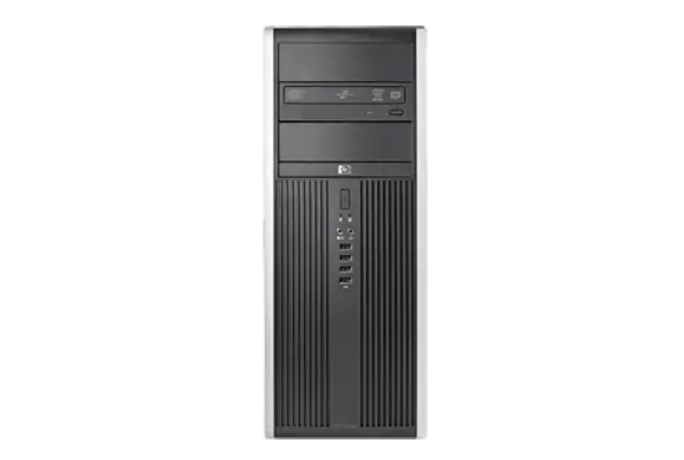
\includegraphics[width=0.25\textwidth,height=4cm,keepaspectratio]{tablas-images/cp1/torres/torre-1.png}} \\ \cline{1-1}
\textbf{MODELO:} Desconocido & \\ \cline{1-1}
\textbf{MARCA:} HP & \\ \cline{1-1}
\textbf{CÓDIGO DE INVENTARIO:} 7 24390 49879 4 & \\ \cline{1-1}
\textbf{NÚMERO EN CPD:} 14 & \\ \hline
\multicolumn{2}{|l|}{\textbf{ESPECIFICACIONES TÉCNICAS}} \\ \hline
\multicolumn{2}{|p{0.95\textwidth}|}{
\footnotesize
- 8 entradas USB (4 al frente, 4 en la parte trasera)
- Entrada de audio y microfono
- Entrada HDMI
- Lector de DVDs
- 3 puertos Ethernet (Parte trasera)
- Entrada Displayport
- Puertos PS/2 (Teclado y Ratón)
} \\ \hline
\multicolumn{2}{|l|}{\textbf{PROPÓSITO:} Hipervisor de XCP-ng} \\ \hline
\multicolumn{2}{|l|}{\textbf{OPORTUNIDAD DE USO:} Proyectos del \GRID} \\ \hline
\multicolumn{2}{|p{0.9\textwidth}|}{\textbf{OBSERVACIONES:} El Equipo no tiene modelo. El equipo está diseñado para usuario final pero fue adaptado para entornos de virtualización.} \\ \hline
\end{tabular}
\end{table}

% Torre 5
\begin{table}[H]
\centering
\caption{Ficha técnica --- Torre 5}
\label{tab:torre-5}
\begin{tabular}{|p{0.6\textwidth}|p{0.3\textwidth}|}
\hline
\multicolumn{2}{|l|}{\textbf{DESCRIPCIÓN FÍSICA:} Servidor tipo torre} \\ \hline
\textbf{TIPO DE RECURSO:} Torre & 
\multirow{5}{*}{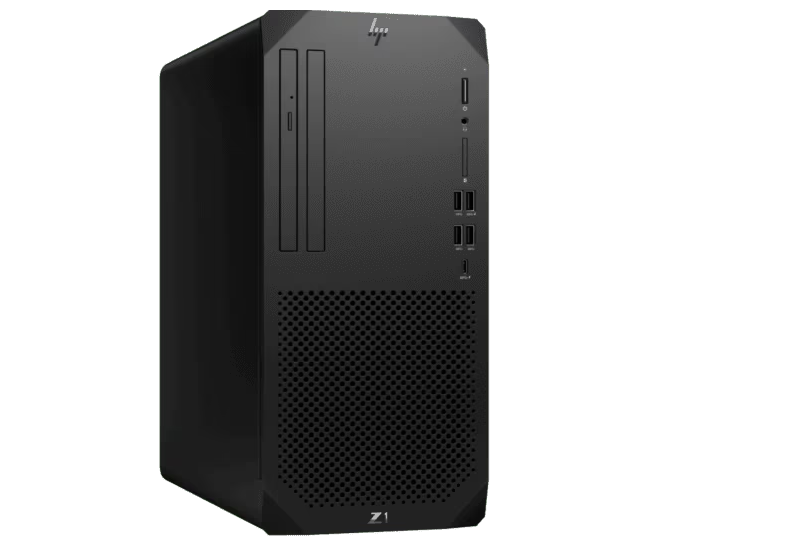
\includegraphics[width=0.25\textwidth,height=4cm,keepaspectratio]{tablas-images/cp1/torres/torre-2.png}} \\ \cline{1-1}
\textbf{MODELO:} G9 & \\ \cline{1-1}
\textbf{MARCA:} HP & \\ \cline{1-1}
\textbf{CÓDIGO DE INVENTARIO:} 72992 & \\ \cline{1-1}
\textbf{NÚMERO EN CPD:} 22 & \\ \hline
\multicolumn{2}{|l|}{\textbf{ESPECIFICACIONES TÉCNICAS}} \\ \hline
\multicolumn{2}{|p{0.95\textwidth}|}{
\footnotesize
- 9 entradas USB (4 al frente, 5 en la parte trasera)
- Entrada de audio y microfono
- Entrada HDMI
- Lector de DVDs
- 1 puerto Ethernet (Parte trasera)
- 2 Entrada Displayport
- Procesador Intel vPro i9
} \\ \hline
\multicolumn{2}{|l|}{\textbf{PROPÓSITO:} Hipervisor de XCP-ng} \\ \hline
\multicolumn{2}{|l|}{\textbf{OPORTUNIDAD DE USO:} Proyectos del \GRID} \\ \hline
\multicolumn{2}{|p{0.9\textwidth}|}{\textbf{OBSERVACIONES:} El equipo está diseñado para usuario final pero fue adaptado para entornos de virtualización.} \\ \hline
\end{tabular}
\end{table}

% Torre 6
\begin{table}[H]
\centering
\caption{Ficha técnica --- Torre 6}
\label{tab:torre-6}
\begin{tabular}{|p{0.6\textwidth}|p{0.3\textwidth}|}
\hline
\multicolumn{2}{|l|}{\textbf{DESCRIPCIÓN FÍSICA:} Servidor tipo torre} \\ \hline
\textbf{TIPO DE RECURSO:} Torre & 
\multirow{5}{*}{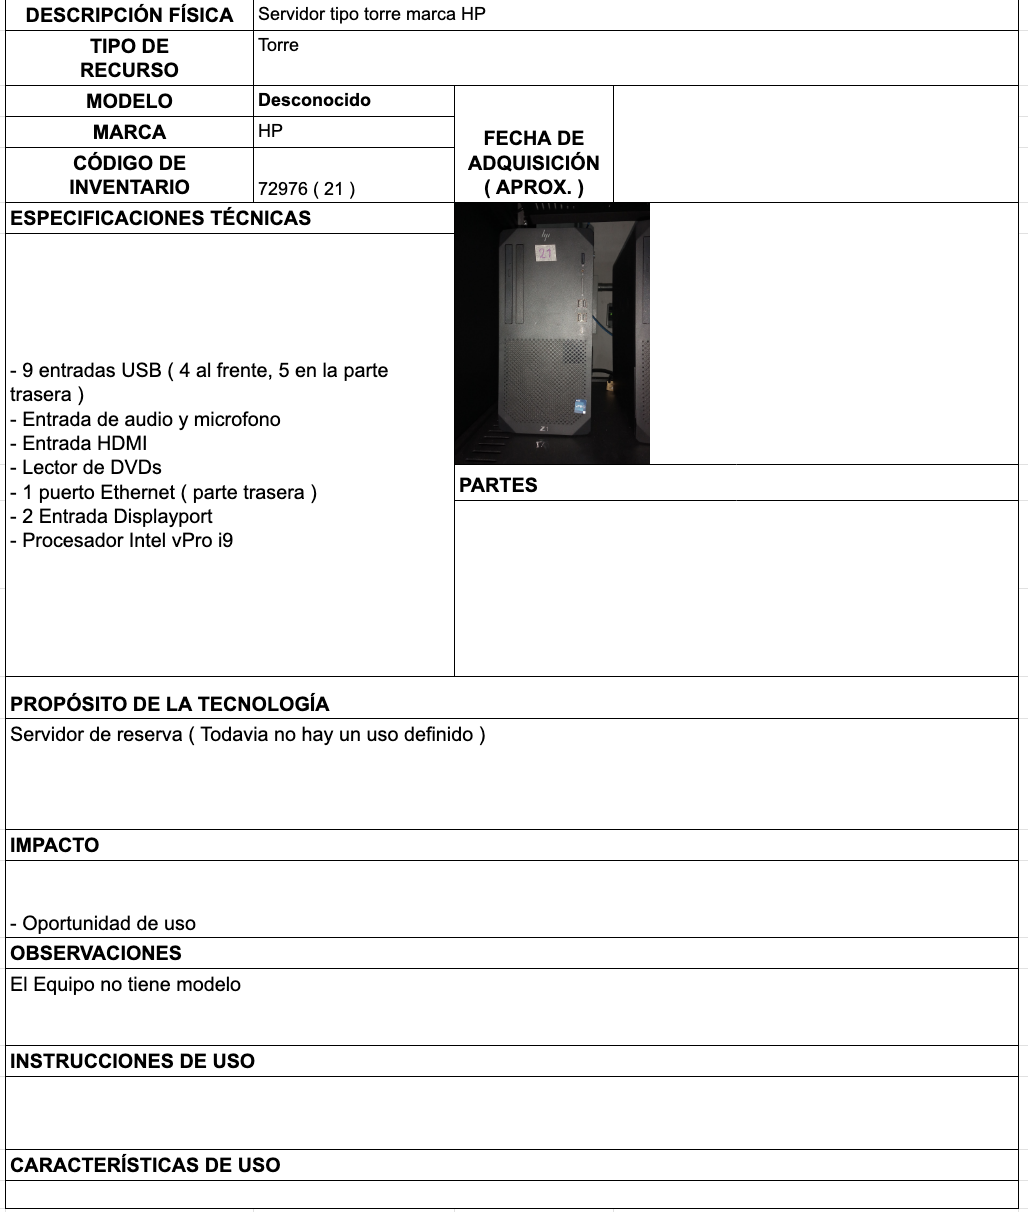
\includegraphics[width=0.25\textwidth,height=4cm,keepaspectratio]{tablas-images/cp1/torres/torre-6.png}} \\ \cline{1-1}
\textbf{MODELO:} Por definir & \\ \cline{1-1}
\textbf{MARCA:} Por definir & \\ \cline{1-1}
\textbf{CÓDIGO DE INVENTARIO:} Por definir & \\ \cline{1-1}
\textbf{FECHA DE ADQUISICIÓN (APROX.):} & \\ \hline
\multicolumn{2}{|l|}{\textbf{ESPECIFICACIONES TÉCNICAS}} \\ \hline
\multicolumn{2}{|p{0.95\textwidth}|}{
\footnotesize
Especificaciones por definir según imagen adjunta
} \\ \hline
\multicolumn{2}{|l|}{\textbf{PROPÓSITO:} Por definir} \\ \hline
\multicolumn{2}{|l|}{\textbf{IMPACTO:} Por evaluar} \\ \hline
\multicolumn{2}{|l|}{\textbf{OBSERVACIONES:} Ver imagen para detalles} \\ \hline
\end{tabular}
\end{table}

% Torre 7
\begin{table}[H]
\centering
\caption{Ficha técnica -- Torre 7}
\label{tab:torre-7}
\begin{tabular}{|p{0.6\textwidth}|p{0.3\textwidth}|}
\hline
\multicolumn{2}{|l|}{\textbf{DESCRIPCIÓN FÍSICA:} Servidor tipo torre} \\ \hline
\textbf{TIPO DE RECURSO:} Torre & 
\multirow{5}{*}{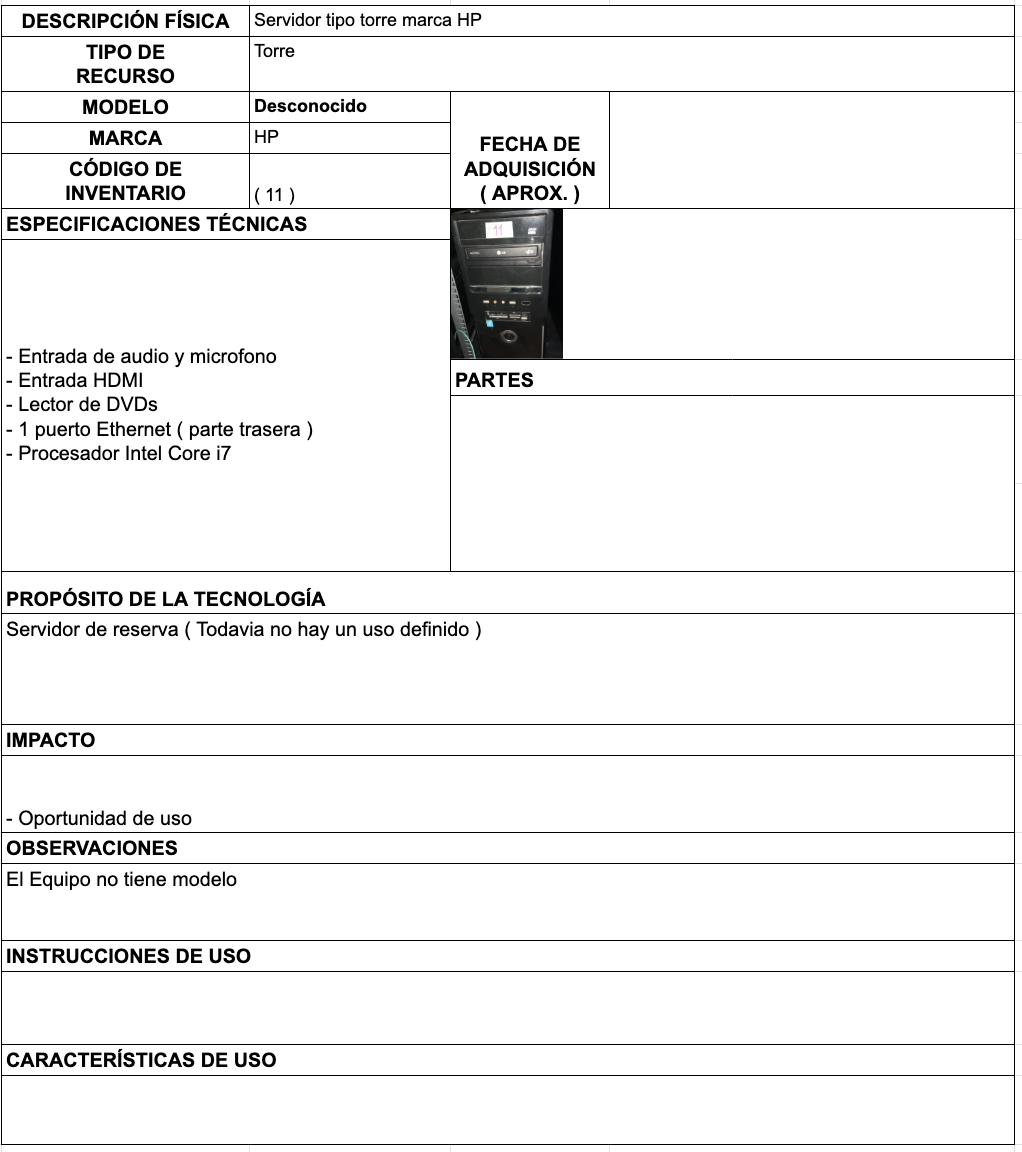
\includegraphics[width=0.25\textwidth,height=4cm,keepaspectratio]{tablas-images/cp1/torres/torre-7.png}} \\ \cline{1-1}
\textbf{MODELO:} Por definir & \\ \cline{1-1}
\textbf{MARCA:} Por definir & \\ \cline{1-1}
\textbf{CÓDIGO DE INVENTARIO:} Por definir & \\ \cline{1-1}
\textbf{FECHA DE ADQUISICIÓN (APROX.):} & \\ \hline
\multicolumn{2}{|l|}{\textbf{ESPECIFICACIONES TÉCNICAS}} \\ \hline
\multicolumn{2}{|p{0.95\textwidth}|}{
\footnotesize
Especificaciones por definir según imagen adjunta
} \\ \hline
\multicolumn{2}{|l|}{\textbf{PROPÓSITO:} Por definir} \\ \hline
\multicolumn{2}{|l|}{\textbf{IMPACTO:} Por evaluar} \\ \hline
\multicolumn{2}{|l|}{\textbf{OBSERVACIONES:} Ver imagen para detalles} \\ \hline
\end{tabular}
\end{table}

% Rack 1
\begin{table}[H]
\centering
\caption{Ficha técnica -- Rack 1}
\label{tab:rack-1}
\begin{tabular}{|p{0.6\textwidth}|p{0.3\textwidth}|}
\hline
\multicolumn{2}{|l|}{\textbf{DESCRIPCIÓN FÍSICA:} Servidor tipo rack} \\ \hline
\textbf{TIPO DE RECURSO:} Rack & 
\multirow{5}{*}{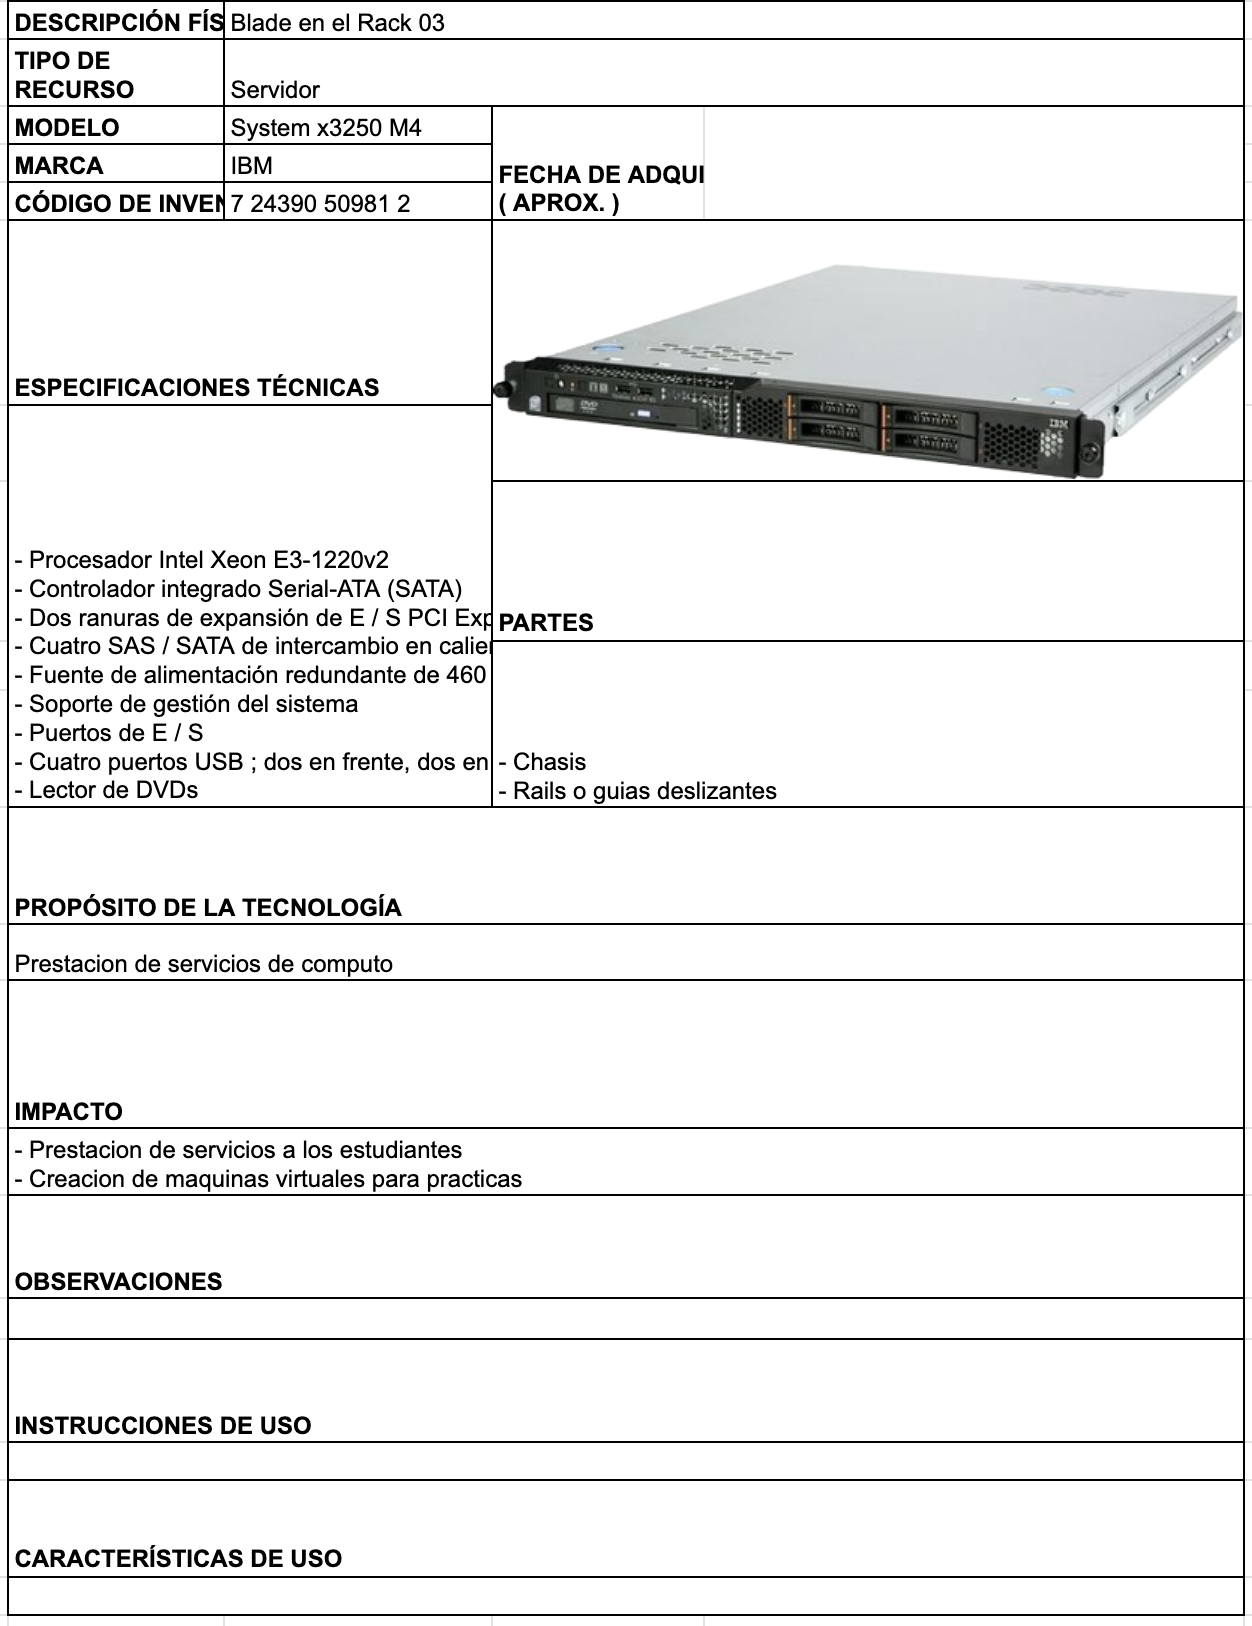
\includegraphics[width=0.25\textwidth,height=4cm,keepaspectratio]{tablas-images/cp1/racks/rack-1.png}} \\ \cline{1-1}
\textbf{MODELO:} Por definir & \\ \cline{1-1}
\textbf{MARCA:} Por definir & \\ \cline{1-1}
\textbf{CÓDIGO DE INVENTARIO:} Por definir & \\ \cline{1-1}
\textbf{FECHA DE ADQUISICIÓN (APROX.):} & \\ \hline
\multicolumn{2}{|l|}{\textbf{ESPECIFICACIONES TÉCNICAS}} \\ \hline
\multicolumn{2}{|p{0.95\textwidth}|}{
\footnotesize
Especificaciones por definir según imagen adjunta
} \\ \hline
\multicolumn{2}{|l|}{\textbf{PROPÓSITO:} Por definir} \\ \hline
\multicolumn{2}{|l|}{\textbf{IMPACTO:} Por evaluar} \\ \hline
\multicolumn{2}{|l|}{\textbf{OBSERVACIONES:} Ver imagen para detalles} \\ \hline
\end{tabular}
\end{table}

% Rack 2
\begin{table}[H]
\centering
\caption{Ficha técnica -- Rack 2}
\label{tab:rack-2}
\begin{tabular}{|p{0.6\textwidth}|p{0.3\textwidth}|}
\hline
\multicolumn{2}{|l|}{\textbf{DESCRIPCIÓN FÍSICA:} Servidor tipo rack} \\ \hline
\textbf{TIPO DE RECURSO:} Rack & 
\multirow{5}{*}{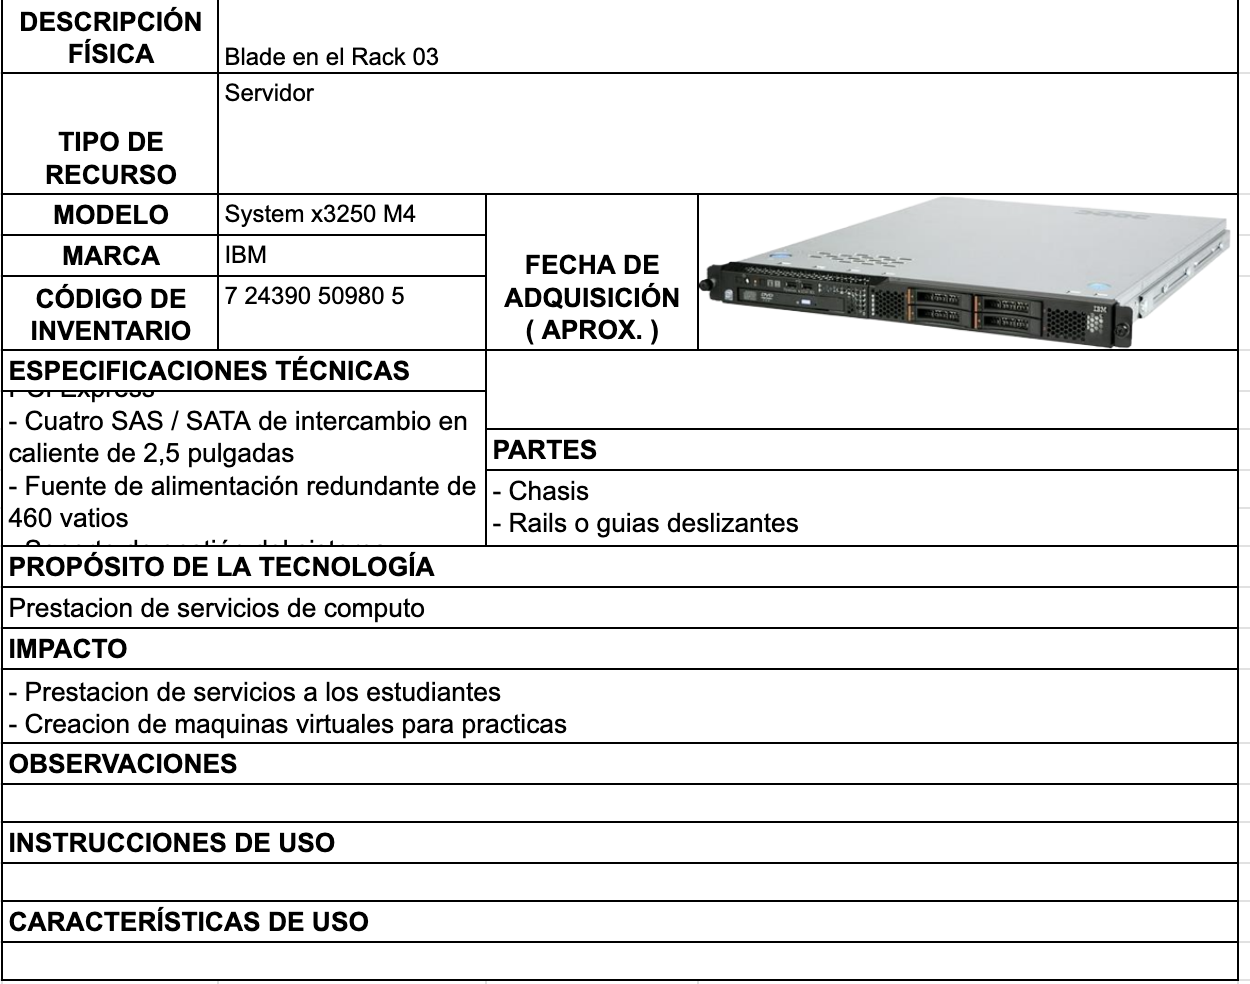
\includegraphics[width=0.25\textwidth,height=4cm,keepaspectratio]{tablas-images/cp1/racks/rack-2.png}} \\ \cline{1-1}
\textbf{MODELO:} Por definir & \\ \cline{1-1}
\textbf{MARCA:} Por definir & \\ \cline{1-1}
\textbf{CÓDIGO DE INVENTARIO:} Por definir & \\ \cline{1-1}
\textbf{FECHA DE ADQUISICIÓN (APROX.):} & \\ \hline
\multicolumn{2}{|l|}{\textbf{ESPECIFICACIONES TÉCNICAS}} \\ \hline
\multicolumn{2}{|p{0.95\textwidth}|}{
\footnotesize
Especificaciones por definir según imagen adjunta
} \\ \hline
\multicolumn{2}{|l|}{\textbf{PROPÓSITO:} Por definir} \\ \hline
\multicolumn{2}{|l|}{\textbf{IMPACTO:} Por evaluar} \\ \hline
\multicolumn{2}{|l|}{\textbf{OBSERVACIONES:} Ver imagen para detalles} \\ \hline
\end{tabular}
\end{table}

% Rack 3
\begin{table}[H]
\centering
\caption{Ficha técnica -- Rack 3}
\label{tab:rack-3}
\begin{tabular}{|p{0.6\textwidth}|p{0.3\textwidth}|}
\hline
\multicolumn{2}{|l|}{\textbf{DESCRIPCIÓN FÍSICA:} Servidor tipo rack} \\ \hline
\textbf{TIPO DE RECURSO:} Rack & 
\multirow{5}{*}{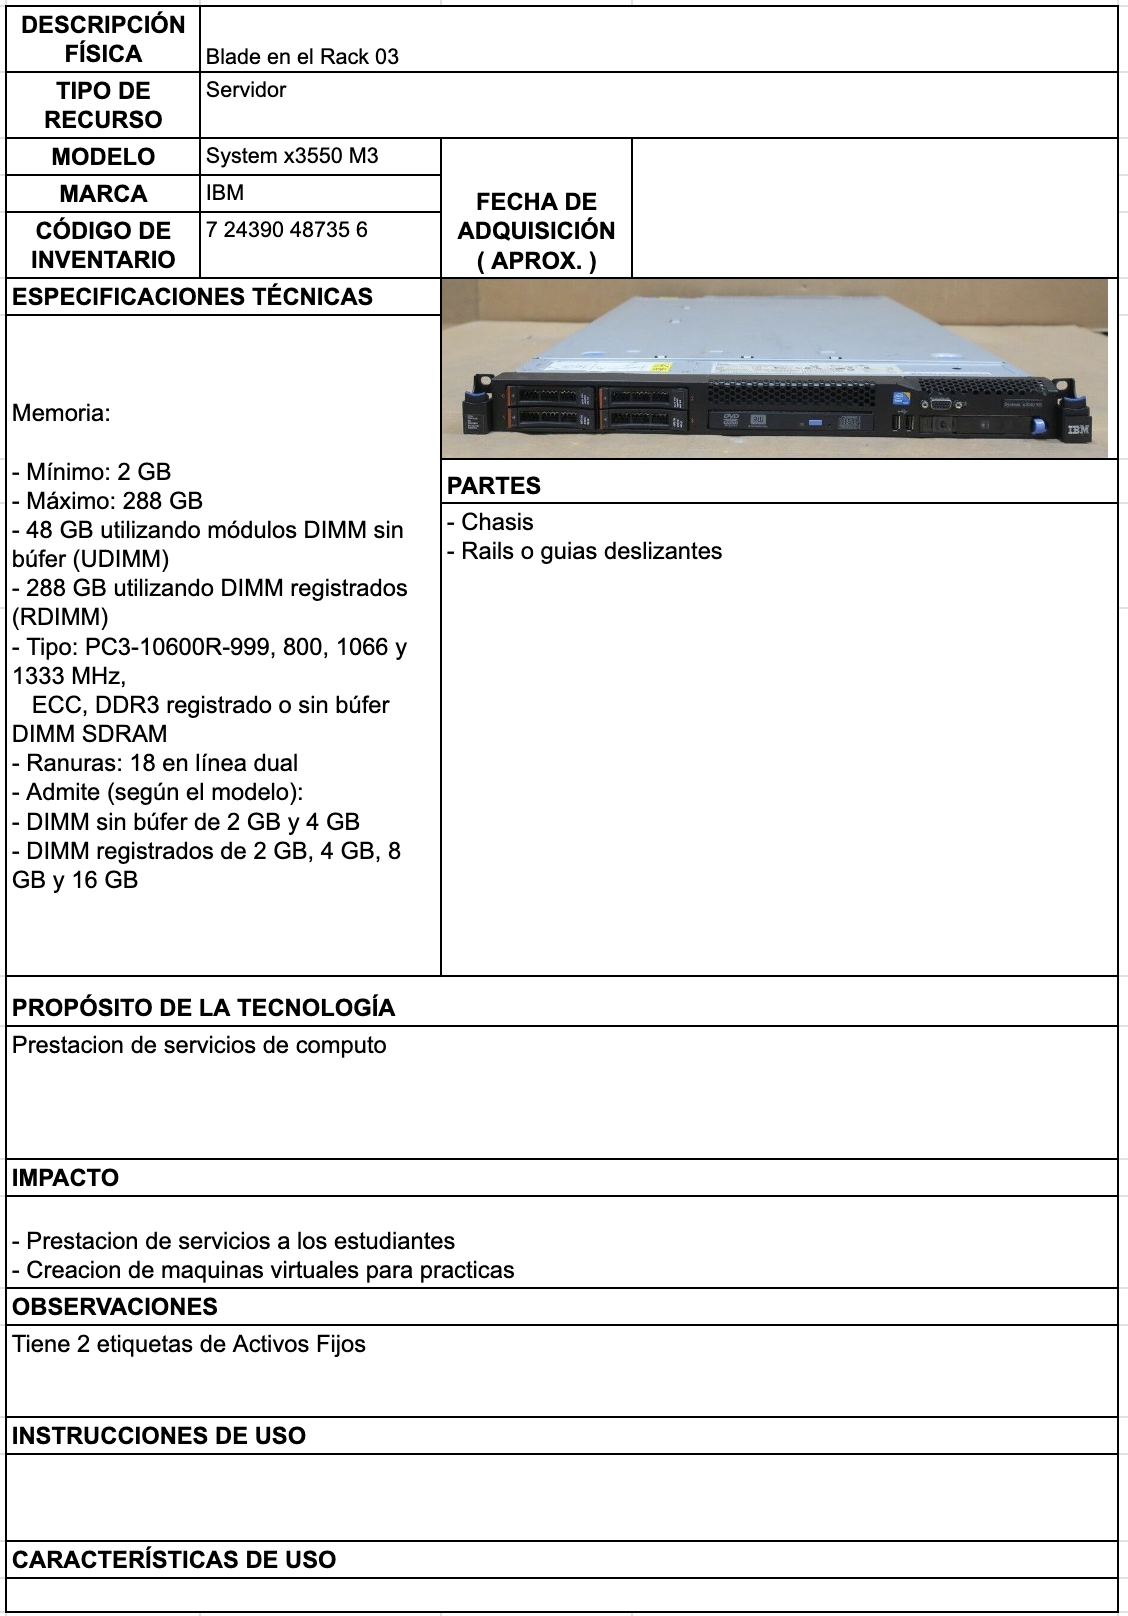
\includegraphics[width=0.25\textwidth,height=4cm,keepaspectratio]{tablas-images/cp1/racks/rack-3.png}} \\ \cline{1-1}
\textbf{MODELO:} Por definir & \\ \cline{1-1}
\textbf{MARCA:} Por definir & \\ \cline{1-1}
\textbf{CÓDIGO DE INVENTARIO:} Por definir & \\ \cline{1-1}
\textbf{FECHA DE ADQUISICIÓN (APROX.):} & \\ \hline
\multicolumn{2}{|l|}{\textbf{ESPECIFICACIONES TÉCNICAS}} \\ \hline
\multicolumn{2}{|p{0.95\textwidth}|}{
\footnotesize
Especificaciones por definir según imagen adjunta
} \\ \hline
\multicolumn{2}{|l|}{\textbf{PROPÓSITO:} Por definir} \\ \hline
\multicolumn{2}{|l|}{\textbf{IMPACTO:} Por evaluar} \\ \hline
\multicolumn{2}{|l|}{\textbf{OBSERVACIONES:} Ver imagen para detalles} \\ \hline
\end{tabular}
\end{table}

% Rack 4
\begin{table}[H]
\centering
\caption{Ficha técnica -- Rack 4}
\label{tab:rack-4}
\begin{tabular}{|p{0.6\textwidth}|p{0.3\textwidth}|}
\hline
\multicolumn{2}{|l|}{\textbf{DESCRIPCIÓN FÍSICA:} Servidor tipo rack} \\ \hline
\textbf{TIPO DE RECURSO:} Rack & 
\multirow{5}{*}{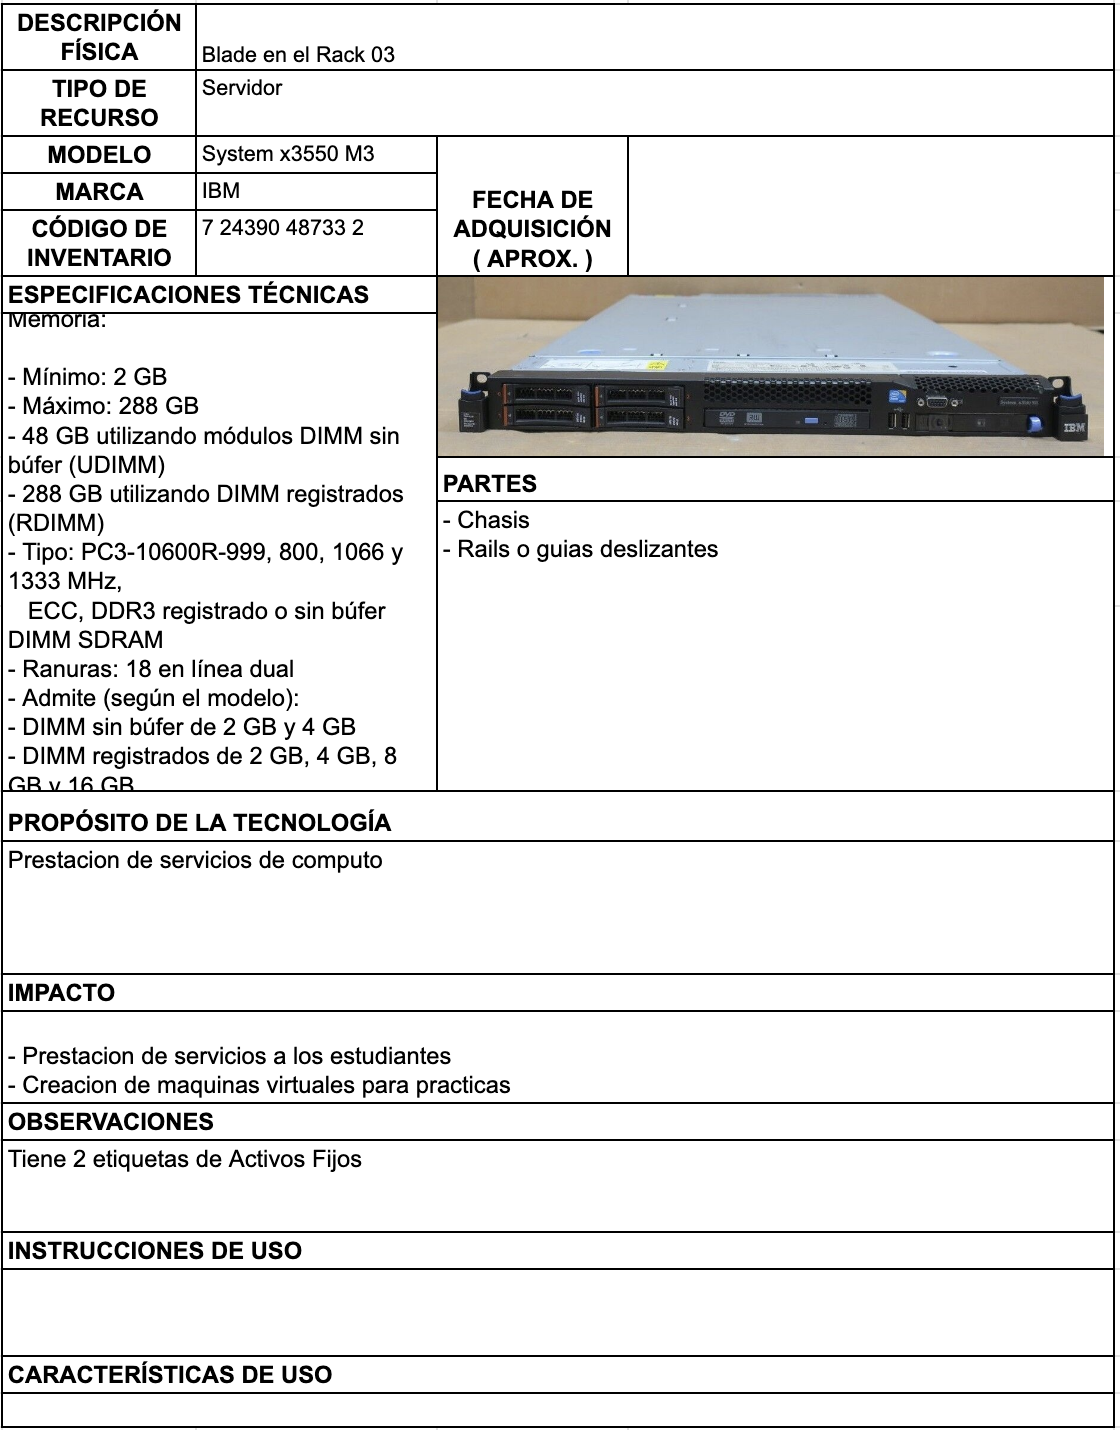
\includegraphics[width=0.25\textwidth,height=4cm,keepaspectratio]{tablas-images/cp1/racks/rack-4.png}} \\ \cline{1-1}
\textbf{MODELO:} Por definir & \\ \cline{1-1}
\textbf{MARCA:} Por definir & \\ \cline{1-1}
\textbf{CÓDIGO DE INVENTARIO:} Por definir & \\ \cline{1-1}
\textbf{FECHA DE ADQUISICIÓN (APROX.):} & \\ \hline
\multicolumn{2}{|l|}{\textbf{ESPECIFICACIONES TÉCNICAS}} \\ \hline
\multicolumn{2}{|p{0.95\textwidth}|}{
\footnotesize
Especificaciones por definir según imagen adjunta
} \\ \hline
\multicolumn{2}{|l|}{\textbf{PROPÓSITO:} Por definir} \\ \hline
\multicolumn{2}{|l|}{\textbf{IMPACTO:} Por evaluar} \\ \hline
\multicolumn{2}{|l|}{\textbf{OBSERVACIONES:} Ver imagen para detalles} \\ \hline
\end{tabular}
\end{table}

% Rack 5
\begin{table}[H]
\centering
\caption{Ficha técnica -- Rack 5}
\label{tab:rack-5}
\begin{tabular}{|p{0.6\textwidth}|p{0.3\textwidth}|}
\hline
\multicolumn{2}{|l|}{\textbf{DESCRIPCIÓN FÍSICA:} Servidor tipo rack} \\ \hline
\textbf{TIPO DE RECURSO:} Rack & 
\multirow{5}{*}{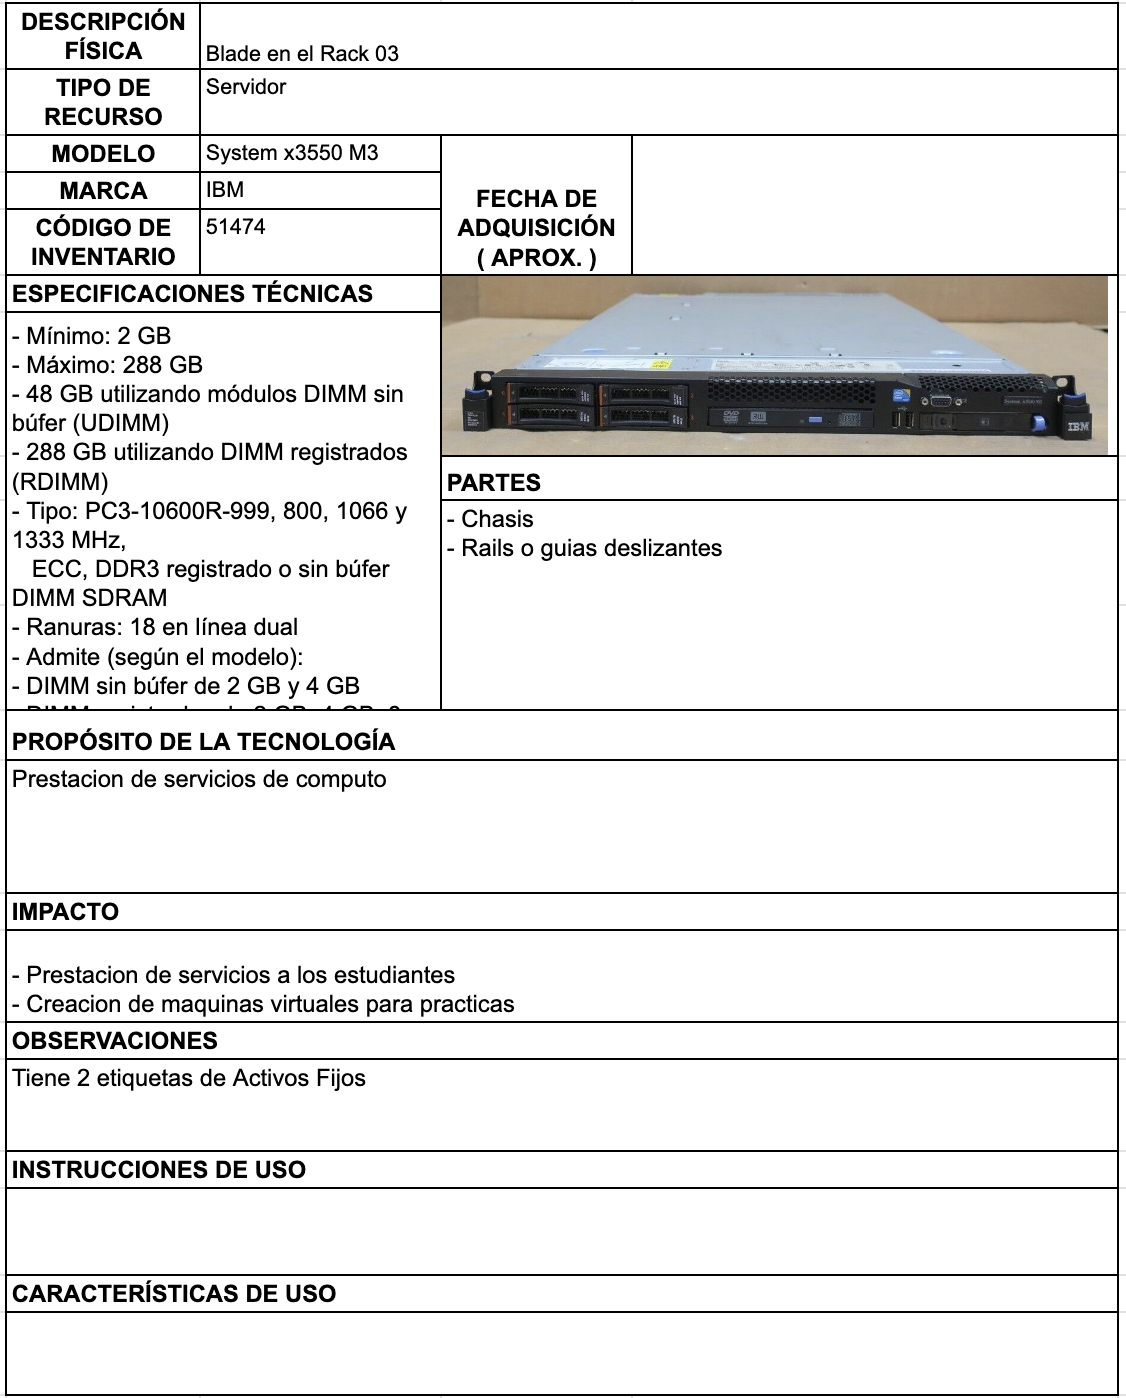
\includegraphics[width=0.25\textwidth,height=4cm,keepaspectratio]{tablas-images/cp1/racks/rack-5.png}} \\ \cline{1-1}
\textbf{MODELO:} Por definir & \\ \cline{1-1}
\textbf{MARCA:} Por definir & \\ \cline{1-1}
\textbf{CÓDIGO DE INVENTARIO:} Por definir & \\ \cline{1-1}
\textbf{FECHA DE ADQUISICIÓN (APROX.):} & \\ \hline
\multicolumn{2}{|l|}{\textbf{ESPECIFICACIONES TÉCNICAS}} \\ \hline
\multicolumn{2}{|p{0.95\textwidth}|}{
\footnotesize
Especificaciones por definir según imagen adjunta
} \\ \hline
\multicolumn{2}{|l|}{\textbf{PROPÓSITO:} Por definir} \\ \hline
\multicolumn{2}{|l|}{\textbf{IMPACTO:} Por evaluar} \\ \hline
\multicolumn{2}{|l|}{\textbf{OBSERVACIONES:} Ver imagen para detalles} \\ \hline
\end{tabular}
\end{table}

% NAS 1
\begin{table}[H]
\centering
\caption{Ficha técnica -- NAS 1}
\label{tab:nas-1}
\begin{tabular}{|p{0.6\textwidth}|p{0.3\textwidth}|}
\hline
\multicolumn{2}{|l|}{\textbf{DESCRIPCIÓN FÍSICA:} Sistema de almacenamiento conectado en red} \\ \hline
\textbf{TIPO DE RECURSO:} NAS (Network Attached Storage) & 
\multirow{5}{*}{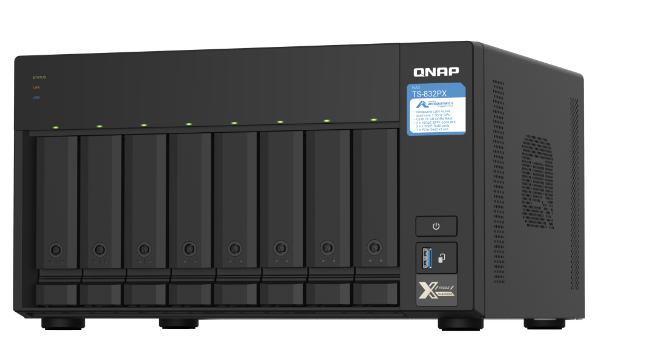
\includegraphics[width=0.25\textwidth,height=4cm,keepaspectratio]{tablas-images/cp1/NAS/nas-1.png}} \\ \cline{1-1}
\textbf{MODELO:} Por definir & \\ \cline{1-1}
\textbf{MARCA:} Por definir & \\ \cline{1-1}
\textbf{CÓDIGO DE INVENTARIO:} Por definir & \\ \cline{1-1}
\textbf{FECHA DE ADQUISICIÓN (APROX.):} & \\ \hline
\multicolumn{2}{|l|}{\textbf{ESPECIFICACIONES TÉCNICAS}} \\ \hline
\multicolumn{2}{|p{0.95\textwidth}|}{
\footnotesize
Especificaciones por definir según imagen adjunta
} \\ \hline
\multicolumn{2}{|l|}{\textbf{PROPÓSITO:} Por definir} \\ \hline
\multicolumn{2}{|l|}{\textbf{IMPACTO:} Por evaluar} \\ \hline
\multicolumn{2}{|l|}{\textbf{OBSERVACIONES:} Ver imagen para detalles} \\ \hline
\end{tabular}
\end{table}

% Firewall 1
\begin{table}[H]
\centering
\caption{Ficha técnica -- Firewall 1}
\label{tab:firewall-1}
\begin{tabular}{|p{0.6\textwidth}|p{0.3\textwidth}|}
\hline
\multicolumn{2}{|l|}{\textbf{DESCRIPCIÓN FÍSICA:} Sistema de seguridad de red} \\ \hline
\textbf{TIPO DE RECURSO:} Firewall & 
\multirow{5}{*}{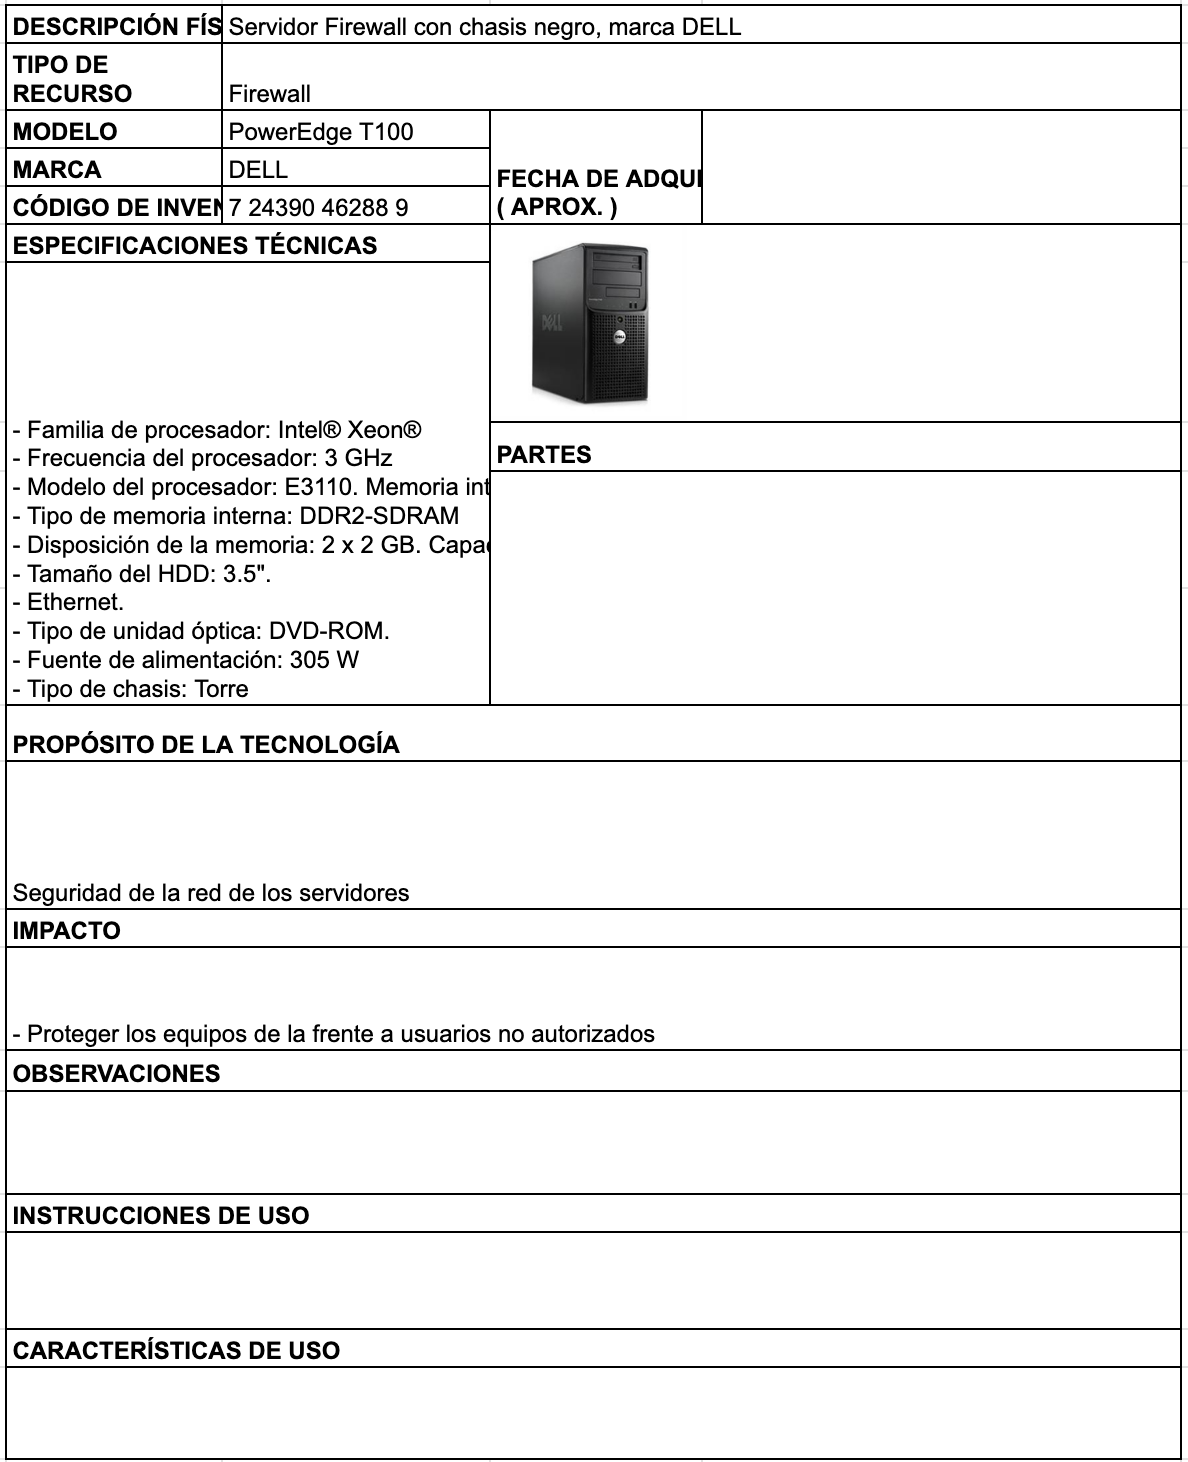
\includegraphics[width=0.25\textwidth,height=4cm,keepaspectratio]{tablas-images/cp1/firewall/firewall.png}} \\ \cline{1-1}
\textbf{MODELO:} Por definir & \\ \cline{1-1}
\textbf{MARCA:} Por definir & \\ \cline{1-1}
\textbf{CÓDIGO DE INVENTARIO:} Por definir & \\ \cline{1-1}
\textbf{FECHA DE ADQUISICIÓN (APROX.):} & \\ \hline
\multicolumn{2}{|l|}{\textbf{ESPECIFICACIONES TÉCNICAS}} \\ \hline
\multicolumn{2}{|p{0.95\textwidth}|}{
\footnotesize
Especificaciones por definir según imagen adjunta
} \\ \hline
\multicolumn{2}{|l|}{\textbf{PROPÓSITO:} Por definir} \\ \hline
\multicolumn{2}{|l|}{\textbf{IMPACTO:} Por evaluar} \\ \hline
\multicolumn{2}{|l|}{\textbf{OBSERVACIONES:} Ver imagen para detalles} \\ \hline
\end{tabular}
\end{table}